\chapter{The Promise}

It was indeed Maximilian Morrel, who had passed a wretched existence
since the previous day. With the instinct peculiar to lovers he had
anticipated after the return of Madame de Saint-Méran and the death of
the marquis, that something would occur at M. de Villefort’s in
connection with his attachment for Valentine. His presentiments were
realized, as we shall see, and his uneasy forebodings had goaded him
pale and trembling to the gate under the chestnut-trees.

Valentine was ignorant of the cause of this sorrow and anxiety, and as
it was not his accustomed hour for visiting her, she had gone to the
spot simply by accident or perhaps through sympathy. Morrel called her,
and she ran to the gate.

“You here at this hour?” said she.

“Yes, my poor girl,” replied Morrel; “I come to bring and to hear bad
tidings.”

“This is, indeed, a house of mourning,” said Valentine; “speak,
Maximilian, although the cup of sorrow seems already full.”

“Dear Valentine,” said Morrel, endeavoring to conceal his own emotion,
“listen, I entreat you; what I am about to say is very serious. When
are you to be married?”

“I will tell you all,” said Valentine; “from you I have nothing to
conceal. This morning the subject was introduced, and my dear
grandmother, on whom I depended as my only support, not only declared
herself favorable to it, but is so anxious for it, that they only await
the arrival of M. d’Épinay, and the following day the contract will be
signed.”

A deep sigh escaped the young man, who gazed long and mournfully at her
he loved.

“Alas,” replied he, “it is dreadful thus to hear my condemnation from
your own lips. The sentence is passed, and, in a few hours, will be
executed; it must be so, and I will not endeavor to prevent it. But,
since you say nothing remains but for M. d’Épinay to arrive that the
contract may be signed, and the following day you will be his, tomorrow
you will be engaged to M. d’Épinay, for he came this morning to Paris.”
Valentine uttered a cry.

“I was at the house of Monte Cristo an hour since,” said Morrel; “we
were speaking, he of the sorrow your family had experienced, and I of
your grief, when a carriage rolled into the courtyard. Never, till
then, had I placed any confidence in presentiments, but now I cannot
help believing them, Valentine. At the sound of that carriage I
shuddered; soon I heard steps on the staircase, which terrified me as
much as the footsteps of the commander did Don Juan. The door at last
opened; Albert de Morcerf entered first, and I began to hope my fears
were vain, when, after him, another young man advanced, and the count
exclaimed: ‘Ah, here is the Baron Franz d’Épinay!’ I summoned all my
strength and courage to my support. Perhaps I turned pale and trembled,
but certainly I smiled; and five minutes after I left, without having
heard one word that had passed.”

“Poor Maximilian!” murmured Valentine.

“Valentine, the time has arrived when you must answer me. And remember
my life depends on your answer. What do you intend doing?” Valentine
held down her head; she was overwhelmed.

“Listen,” said Morrel; “it is not the first time you have contemplated
our present position, which is a serious and urgent one; I do not think
it is a moment to give way to useless sorrow; leave that for those who
like to suffer at their leisure and indulge their grief in secret.
There are such in the world, and God will doubtless reward them in
heaven for their resignation on earth, but those who mean to contend
must not lose one precious moment, but must return immediately the blow
which fortune strikes. Do you intend to struggle against our
ill-fortune? Tell me, Valentine for it is that I came to know.”

Valentine trembled, and looked at him with amazement. The idea of
resisting her father, her grandmother, and all the family, had never
occurred to her.

“What do you say, Maximilian?” asked Valentine. “What do you mean by a
struggle? Oh, it would be a sacrilege. What? I resist my father’s
order, and my dying grandmother’s wish? Impossible!”

Morrel started.

“You are too noble not to understand me, and you understand me so well
that you already yield, dear Maximilian. No, no; I shall need all my
strength to struggle with myself and support my grief in secret, as you
say. But to grieve my father—to disturb my grandmother’s last
moments—never!”

“You are right,” said Morrel, calmly.

“In what a tone you speak!” cried Valentine.

“I speak as one who admires you, mademoiselle.”

“Mademoiselle,” cried Valentine; “mademoiselle! Oh, selfish man! he
sees me in despair, and pretends he cannot understand me!”

“You mistake—I understand you perfectly. You will not oppose M.
Villefort, you will not displease the marchioness, and tomorrow you
will sign the contract which will bind you to your husband.”

“But, \textit{mon Dieu!} tell me, how can I do otherwise?”

“Do not appeal to me, mademoiselle; I shall be a bad judge in such a
case; my selfishness will blind me,” replied Morrel, whose low voice
and clenched hands announced his growing desperation.

“What would you have proposed, Maximilian, had you found me willing to
accede?”

“It is not for me to say.”

“You are wrong; you must advise me what to do.”

“Do you seriously ask my advice, Valentine?”

“Certainly, dear Maximilian, for if it is good, I will follow it; you
know my devotion to you.”

“Valentine,” said Morrel pushing aside a loose plank, “give me your
hand in token of forgiveness of my anger; my senses are confused, and
during the last hour the most extravagant thoughts have passed through
my brain. Oh, if you refuse my advice——”

“What do you advise?” said Valentine, raising her eyes to heaven and
sighing.

“I am free,” replied Maximilian, “and rich enough to support you. I
swear to make you my lawful wife before my lips even shall have
approached your forehead.”

“You make me tremble!” said the young girl.

“Follow me,” said Morrel; “I will take you to my sister, who is worthy
also to be yours. We will embark for Algiers, for England, for America,
or, if you prefer it, retire to the country and only return to Paris
when our friends have reconciled your family.”

Valentine shook her head.

“I feared it, Maximilian,” said she; “it is the counsel of a madman,
and I should be more mad than you, did I not stop you at once with the
word ‘Impossible, Morrel, impossible!’”

“You will then submit to what fate decrees for you without even
attempting to contend with it?” said Morrel sorrowfully.

“Yes,—if I die!”

“Well, Valentine,” resumed Maximilian, “I can only say again that you
are right. Truly, it is I who am mad, and you prove to me that passion
blinds the most well-meaning. I appreciate your calm reasoning. It is
then understood that tomorrow you will be irrevocably promised to M.
Franz d’Épinay, not only by that theatrical formality invented to
heighten the effect of a comedy called the signature of the contract,
but your own will?”

“Again you drive me to despair, Maximilian,” said Valentine, “again you
plunge the dagger into the wound! What would you do, tell me, if your
sister listened to such a proposition?”

“Mademoiselle,” replied Morrel with a bitter smile, “I am selfish—you
have already said so—and as a selfish man I think not of what others
would do in my situation, but of what I intend doing myself. I think
only that I have known you not a whole year. From the day I first saw
you, all my hopes of happiness have been in securing your affection.
One day you acknowledged that you loved me, and since that day my hope
of future happiness has rested on obtaining you, for to gain you would
be life to me. Now, I think no more; I say only that fortune has turned
against me—I had thought to gain heaven, and now I have lost it. It is
an every-day occurrence for a gambler to lose not only what he
possesses but also what he has not.”

Morrel pronounced these words with perfect calmness; Valentine looked
at him a moment with her large, scrutinizing eyes, endeavoring not to
let Morrel discover the grief which struggled in her heart.

“But, in a word, what are you going to do?” asked she.

“I am going to have the honor of taking my leave of you, mademoiselle,
solemnly assuring you that I wish your life may be so calm, so happy,
and so fully occupied, that there may be no place for me even in your
memory.”

“Oh!” murmured Valentine.

“Adieu, Valentine, adieu!” said Morrel, bowing.

“Where are you going?” cried the young girl, extending her hand through
the opening, and seizing Maximilian by his coat, for she understood
from her own agitated feelings that her lover’s calmness could not be
real; “where are you going?”

“I am going, that I may not bring fresh trouble into your family: and
to set an example which every honest and devoted man, situated as I am,
may follow.”

“Before you leave me, tell me what you are going to do, Maximilian.”
The young man smiled sorrowfully.

“Speak, speak!” said Valentine; “I entreat you.”

“Has your resolution changed, Valentine?”

“It cannot change, unhappy man; you know it must not!” cried the young
girl.

“Then adieu, Valentine!”

Valentine shook the gate with a strength of which she could not have
been supposed to be possessed, as Morrel was going away, and passing
both her hands through the opening, she clasped and wrung them. “I must
know what you mean to do!” said she. “Where are you going?”

“Oh, fear not,” said Maximilian, stopping at a short distance, “I do
not intend to render another man responsible for the rigorous fate
reserved for me. Another might threaten to seek M. Franz, to provoke
him, and to fight with him; all that would be folly. What has M. Franz
to do with it? He saw me this morning for the first time, and has
already forgotten he has seen me. He did not even know I existed when
it was arranged by your two families that you should be united. I have
no enmity against M. Franz, and promise you the punishment shall not
fall on him.”

“On whom, then!—on me?”

“On you? Valentine! Oh, Heaven forbid! Woman is sacred; the woman one
loves is holy.”

“On yourself, then, unhappy man; on yourself?”

“I am the only guilty person, am I not?” said Maximilian.

“Maximilian!” said Valentine, “Maximilian, come back, I entreat you!”

He drew near with his sweet smile, and but for his paleness one might
have thought him in his usual happy mood.

“Listen, my dear, my adored Valentine,” said he in his melodious and
grave tone; “those who, like us, have never had a thought for which we
need blush before the world, such may read each other’s hearts. I never
was romantic, and am no melancholy hero. I imitate neither Manfred nor
Anthony; but without words, protestations, or vows, my life has
entwined itself with yours; you leave me, and you are right in doing
so,—I repeat it, you are right; but in losing you, I lose my life. The
moment you leave me, Valentine, I am alone in the world. My sister is
happily married; her husband is only my brother-in-law, that is, a man
whom the ties of social life alone attach to me; no one then longer
needs my useless life. This is what I shall do; I will wait until the
very moment you are married, for I will not lose the shadow of one of
those unexpected chances which are sometimes reserved for us, since M.
Franz may, after all, die before that time, a thunderbolt may fall even
on the altar as you approach it,—nothing appears impossible to one
condemned to die, and miracles appear quite reasonable when his escape
from death is concerned. I will, then, wait until the last moment, and
when my misery is certain, irremediable, hopeless, I will write a
confidential letter to my brother-in-law, another to the prefect of
police, to acquaint them with my intention, and at the corner of some
wood, on the brink of some abyss, on the bank of some river, I will put
an end to my existence, as certainly as I am the son of the most honest
man who ever lived in France.”

\begin{figure}[ht]
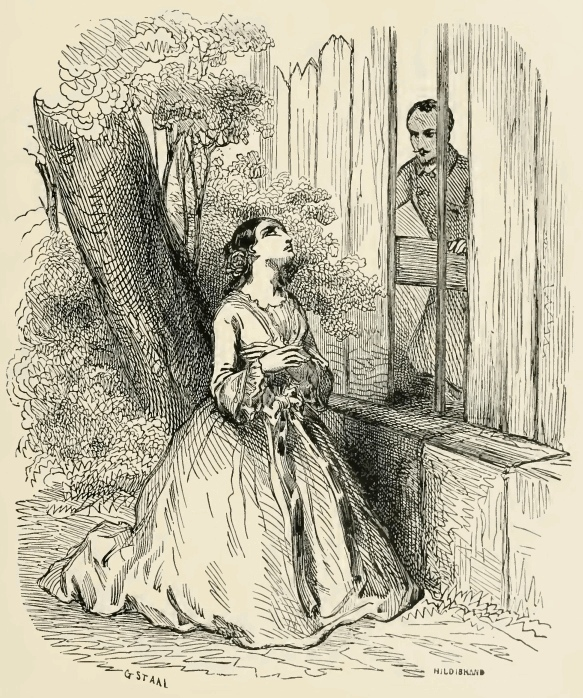
\includegraphics[width=\textwidth]{30333m.jpg}
\end{figure}

Valentine trembled convulsively; she loosened her hold of the gate, her
arms fell by her side, and two large tears rolled down her cheeks. The
young man stood before her, sorrowful and resolute.

“Oh, for pity’s sake,” said she, “you will live, will you not?”

“No, on my honor,” said Maximilian; “but that will not affect you. You
have done your duty, and your conscience will be at rest.”

Valentine fell on her knees, and pressed her almost bursting heart.
“Maximilian,” said she, “Maximilian, my friend, my brother on earth, my
true husband in heaven, I entreat you, do as I do, live in suffering;
perhaps we may one day be united.”

“Adieu, Valentine,” repeated Morrel.

“My God,” said Valentine, raising both her hands to heaven with a
sublime expression, “I have done my utmost to remain a submissive
daughter; I have begged, entreated, implored; he has regarded neither
my prayers, my entreaties, nor my tears. It is done,” cried she, wiping
away her tears, and resuming her firmness, “I am resolved not to die of
remorse, but rather of shame. Live, Maximilian, and I will be yours.
Say when shall it be? Speak, command, I will obey.”

Morrel, who had already gone some few steps away, again returned, and
pale with joy extended both hands towards Valentine through the
opening.

“Valentine,” said he, “dear Valentine, you must not speak thus—rather
let me die. Why should I obtain you by violence, if our love is mutual?
Is it from mere humanity you bid me live? I would then rather die.”

“Truly,” murmured Valentine, “who on this earth cares for me, if he
does not? Who has consoled me in my sorrow but he? On whom do my hopes
rest? On whom does my bleeding heart repose? On him, on him, always on
him! Yes, you are right, Maximilian, I will follow you. I will leave
the paternal home, I will give up all. Oh, ungrateful girl that I am,”
cried Valentine, sobbing, “I will give up all, even my dear old
grandfather, whom I had nearly forgotten.”

“No,” said Maximilian, “you shall not leave him. M. Noirtier has
evinced, you say, a kind feeling towards me. Well, before you leave,
tell him all; his consent would be your justification in God’s sight.
As soon as we are married, he shall come and live with us, instead of
one child, he shall have two. You have told me how you talk to him and
how he answers you; I shall very soon learn that language by signs,
Valentine, and I promise you solemnly, that instead of despair, it is
happiness that awaits us.”

“Oh, see, Maximilian, see the power you have over me, you almost make
me believe you; and yet, what you tell me is madness, for my father
will curse me—he is inflexible—he will never pardon me. Now listen to
me, Maximilian; if by artifice, by entreaty, by accident—in short, if
by any means I can delay this marriage, will you wait?”

“Yes, I promise you, as faithfully as you have promised me that this
horrible marriage shall not take place, and that if you are dragged
before a magistrate or a priest, you will refuse.”

“I promise you by all that is most sacred to me in the world, namely,
by my mother.”

“We will wait, then,” said Morrel.

“Yes, we will wait,” replied Valentine, who revived at these words;
“there are so many things which may save unhappy beings such as we
are.”

“I rely on you, Valentine,” said Morrel; “all you do will be well done;
only if they disregard your prayers, if your father and Madame de
Saint-Méran insist that M. d’Épinay should be called tomorrow to sign
the contract——”

“Then you have my promise, Maximilian.”

“Instead of signing——”

“I will go to you, and we will fly; but from this moment until then,
let us not tempt Providence, let us not see each other. It is a
miracle, it is a providence that we have not been discovered. If we
were surprised, if it were known that we met thus, we should have no
further resource.”

“You are right, Valentine; but how shall I ascertain?”

“From the notary, M. Deschamps.”

“I know him.”

“And for myself—I will write to you, depend on me. I dread this
marriage, Maximilian, as much as you.”

“Thank you, my adored Valentine, thank you; that is enough. When once I
know the hour, I will hasten to this spot, you can easily get over this
fence with my assistance, a carriage will await us at the gate, in
which you will accompany me to my sister’s; there living, retired or
mingling in society, as you wish, we shall be enabled to use our power
to resist oppression, and not suffer ourselves to be put to death like
sheep, which only defend themselves by sighs.”

“Yes,” said Valentine, “I will now acknowledge you are right,
Maximilian; and now are you satisfied with your betrothal?” said the
young girl sorrowfully.

“My adored Valentine, words cannot express one half of my
satisfaction.”

Valentine had approached, or rather, had placed her lips so near the
fence, that they nearly touched those of Morrel, which were pressed
against the other side of the cold and inexorable barrier.

“Adieu, then, till we meet again,” said Valentine, tearing herself
away. “I shall hear from you?”

“Yes.”

“Thanks, thanks, dear love, adieu!”

The sound of a kiss was heard, and Valentine fled through the avenue.
Morrel listened to catch the last sound of her dress brushing the
branches, and of her footstep on the gravel, then raised his eyes with
an ineffable smile of thankfulness to heaven for being permitted to be
thus loved, and then also disappeared.

The young man returned home and waited all the evening and all the next
day without getting any message. It was only on the following day, at
about ten o’clock in the morning, as he was starting to call on M.
Deschamps, the notary, that he received from the postman a small
billet, which he knew to be from Valentine, although he had not before
seen her writing. It was to this effect:

“Tears, entreaties, prayers, have availed me nothing. Yesterday, for
two hours, I was at the church of Saint-Philippe-du-Roule, and for two
hours I prayed most fervently. Heaven is as inflexible as man, and the
signature of the contract is fixed for this evening at nine o’clock. I
have but one promise and but one heart to give; that promise is pledged
to you, that heart is also yours. This evening, then, at a quarter to
nine at the gate.

“Your betrothed,

“Valentine de Villefort.”

“P.S.—My poor grandmother gets worse and worse; yesterday her fever
amounted to delirium; today her delirium is almost madness. You will be
very kind to me, will you not, Morrel, to make me forget my sorrow in
leaving her thus? I think it is kept a secret from grandpapa Noirtier,
that the contract is to be signed this evening.”

Morrel went also to the notary, who confirmed the news that the
contract was to be signed that evening. Then he went to call on Monte
Cristo and heard still more. Franz had been to announce the ceremony,
and Madame de Villefort had also written to beg the count to excuse her
not inviting him; the death of M. de Saint-Méran and the dangerous
illness of his widow would cast a gloom over the meeting which she
would regret should be shared by the count whom she wished every
happiness.

The day before Franz had been presented to Madame de Saint-Méran, who
had left her bed to receive him, but had been obliged to return to it
immediately after.

It is easy to suppose that Morrel’s agitation would not escape the
count’s penetrating eye. Monte Cristo was more affectionate than
ever,—indeed, his manner was so kind that several times Morrel was on
the point of telling him all. But he recalled the promise he had made
to Valentine, and kept his secret.

The young man read Valentine’s letter twenty times in the course of the
day. It was her first, and on what an occasion! Each time he read it he
renewed his vow to make her happy. How great is the power of a woman
who has made so courageous a resolution! What devotion does she deserve
from him for whom she has sacrificed everything! How ought she really
to be supremely loved! She becomes at once a queen and a wife, and it
is impossible to thank and love her sufficiently.

Morrel longed intensely for the moment when he should hear Valentine
say, “Here I am, Maximilian; come and help me.” He had arranged
everything for her escape; two ladders were hidden in the clover-field;
a cabriolet was ordered for Maximilian alone, without a servant,
without lights; at the turning of the first street they would light the
lamps, as it would be foolish to attract the notice of the police by
too many precautions. Occasionally he shuddered; he thought of the
moment when, from the top of that wall, he should protect the descent
of his dear Valentine, pressing in his arms for the first time her of
whom he had yet only kissed the delicate hand.

When the afternoon arrived and he felt that the hour was drawing near,
he wished for solitude, his agitation was extreme; a simple question
from a friend would have irritated him. He shut himself in his room,
and tried to read, but his eye glanced over the page without
understanding a word, and he threw away the book, and for the second
time sat down to sketch his plan, the ladders and the fence.

At length the hour drew near. Never did a man deeply in love allow the
clocks to go on peacefully. Morrel tormented his so effectually that
they struck eight at half-past six. He then said, “It is time to start;
the signature was indeed fixed to take place at nine o’clock, but
perhaps Valentine will not wait for that.” Consequently, Morrel, having
left the Rue Meslay at half-past eight by his timepiece, entered the
clover-field while the clock of Saint-Philippe-du-Roule was striking
eight. The horse and cabriolet were concealed behind a small ruin,
where Morrel had often waited.

The night gradually drew on, and the foliage in the garden assumed a
deeper hue. Then Morrel came out from his hiding-place with a beating
heart, and looked through the small opening in the gate; there was yet
no one to be seen.

The clock struck half-past eight, and still another half-hour was
passed in waiting, while Morrel walked to and fro, and gazed more and
more frequently through the opening. The garden became darker still,
but in the darkness he looked in vain for the white dress, and in the
silence he vainly listened for the sound of footsteps. The house, which
was discernible through the trees, remained in darkness, and gave no
indication that so important an event as the signature of a
marriage-contract was going on. Morrel looked at his watch, which
wanted a quarter to ten; but soon the same clock he had already heard
strike two or three times rectified the error by striking half-past
nine.

This was already half an hour past the time Valentine had fixed. It was
a terrible moment for the young man. The slightest rustling of the
foliage, the least whistling of the wind, attracted his attention, and
drew the perspiration to his brow; then he tremblingly fixed his
ladder, and, not to lose a moment, placed his foot on the first step.
Amidst all these alternations of hope and fear, the clock struck ten.
“It is impossible,” said Maximilian, “that the signing of a contract
should occupy so long a time without unexpected interruptions. I have
weighed all the chances, calculated the time required for all the
forms; something must have happened.”

And then he walked rapidly to and fro, and pressed his burning forehead
against the fence. Had Valentine fainted? or had she been discovered
and stopped in her flight? These were the only obstacles which appeared
possible to the young man.

The idea that her strength had failed her in attempting to escape, and
that she had fainted in one of the paths, was the one that most
impressed itself upon his mind. “In that case,” said he, “I should lose
her, and by my own fault.” He dwelt on this idea for a moment, then it
appeared reality. He even thought he could perceive something on the
ground at a distance; he ventured to call, and it seemed to him that
the wind wafted back an almost inarticulate sigh.

At last the half-hour struck. It was impossible to wait longer, his
temples throbbed violently, his eyes were growing dim; he passed one
leg over the wall, and in a moment leaped down on the other side. He
was on Villefort’s premises—had arrived there by scaling the wall. What
might be the consequences? However, he had not ventured thus far to
draw back. He followed a short distance close under the wall, then
crossed a path, hid entered a clump of trees. In a moment he had passed
through them, and could see the house distinctly.

\begin{figure}[ht]
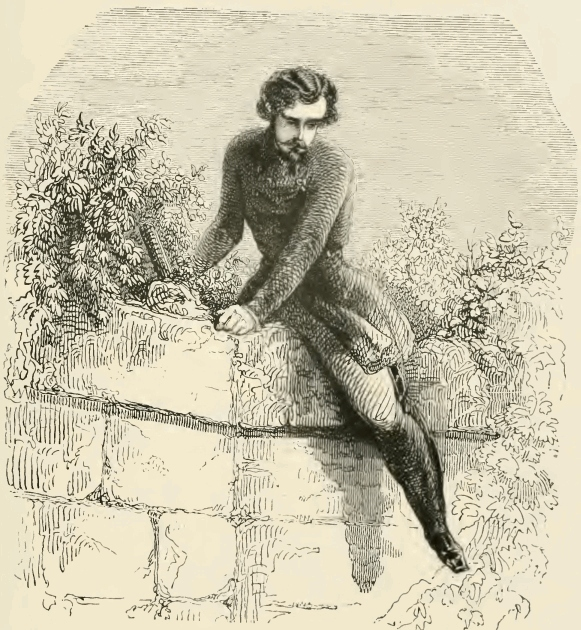
\includegraphics[width=\textwidth]{30341m.jpg}
\end{figure}

Then Morrel saw that he had been right in believing that the house was
not illuminated. Instead of lights at every window, as is customary on
days of ceremony, he saw only a gray mass, which was veiled also by a
cloud, which at that moment obscured the moon’s feeble light. A light
moved rapidly from time to time past three windows of the second floor.
These three windows were in Madame de Saint-Méran’s room. Another
remained motionless behind some red curtains which were in Madame de
Villefort’s bedroom. Morrel guessed all this. So many times, in order
to follow Valentine in thought at every hour in the day, had he made
her describe the whole house, that without having seen it he knew it
all.

This darkness and silence alarmed Morrel still more than Valentine’s
absence had done. Almost mad with grief, and determined to venture
everything in order to see Valentine once more, and be certain of the
misfortune he feared, Morrel gained the edge of the clump of trees, and
was going to pass as quickly as possible through the flower-garden,
when the sound of a voice, still at some distance, but which was borne
upon the wind, reached him. At this sound, as he was already partially
exposed to view, he stepped back and concealed himself completely,
remaining perfectly motionless.

He had formed his resolution. If it was Valentine alone, he would speak
as she passed; if she was accompanied, and he could not speak, still he
should see her, and know that she was safe; if they were strangers, he
would listen to their conversation, and might understand something of
this hitherto incomprehensible mystery.

The moon had just then escaped from behind the cloud which had
concealed it, and Morrel saw Villefort come out upon the steps,
followed by a gentleman in black. They descended, and advanced towards
the clump of trees, and Morrel soon recognized the other gentleman as
Doctor d’Avrigny.

\begin{figure}[ht]
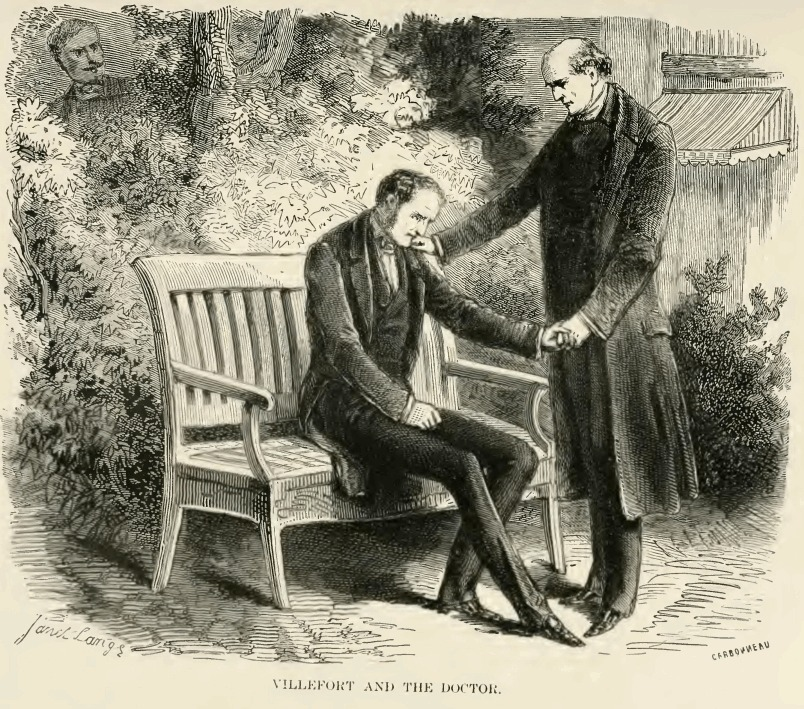
\includegraphics[width=\textwidth]{30339m.jpg}
\end{figure}

The young man, seeing them approach, drew back mechanically, until he
found himself stopped by a sycamore-tree in the centre of the clump;
there he was compelled to remain. Soon the two gentlemen stopped also.

“Ah, my dear doctor,” said the procureur, “Heaven declares itself
against my house! What a dreadful death—what a blow! Seek not to
console me; alas, nothing can alleviate so great a sorrow—the wound is
too deep and too fresh! Dead, dead!”

The cold sweat sprang to the young man’s brow, and his teeth chattered.
Who could be dead in that house, which Villefort himself had called
accursed?

“My dear M. de Villefort,” replied the doctor, with a tone which
redoubled the terror of the young man, “I have not led you here to
console you; on the contrary——”

“What can you mean?” asked the procureur, alarmed.

“I mean that behind the misfortune which has just happened to you,
there is another, perhaps, still greater.”

“Can it be possible?” murmured Villefort, clasping his hands. “What are
you going to tell me?”

“Are we quite alone, my friend?”

“Yes, quite; but why all these precautions?”

“Because I have a terrible secret to communicate to you,” said the
doctor. “Let us sit down.”

Villefort fell, rather than seated himself. The doctor stood before
him, with one hand placed on his shoulder. Morrel, horrified, supported
his head with one hand, and with the other pressed his heart, lest its
beatings should be heard. “Dead, dead!” repeated he within himself; and
he felt as if he were also dying.

“Speak, doctor—I am listening,” said Villefort; “strike—I am prepared
for everything!”

“Madame de Saint-Méran was, doubtless, advancing in years, but she
enjoyed excellent health.” Morrel began again to breathe freely, which
he had not done during the last ten minutes.

“Grief has consumed her,” said Villefort—“yes, grief, doctor! After
living forty years with the marquis——”

“It is not grief, my dear Villefort,” said the doctor; “grief may kill,
although it rarely does, and never in a day, never in an hour, never in
ten minutes.” Villefort answered nothing, he simply raised his head,
which had been cast down before, and looked at the doctor with
amazement.

“Were you present during the last struggle?” asked M. d’Avrigny.

“I was,” replied the procureur; “you begged me not to leave.”

“Did you notice the symptoms of the disease to which Madame de
Saint-Méran has fallen a victim?”

“I did. Madame de Saint-Méran had three successive attacks, at
intervals of some minutes, each one more serious than the former. When
you arrived, Madame de Saint-Méran had already been panting for breath
some minutes; she then had a fit, which I took to be simply a nervous
attack, and it was only when I saw her raise herself in the bed, and
her limbs and neck appear stiffened, that I became really alarmed. Then
I understood from your countenance there was more to fear than I had
thought. This crisis past, I endeavored to catch your eye, but could
not. You held her hand—you were feeling her pulse—and the second fit
came on before you had turned towards me. This was more terrible than
the first; the same nervous movements were repeated, and the mouth
contracted and turned purple.”

“And at the third she expired.”

“At the end of the first attack I discovered symptoms of tetanus; you
confirmed my opinion.”

“Yes, before others,” replied the doctor; “but now we are alone——”

“What are you going to say? Oh, spare me!”

“That the symptoms of tetanus and poisoning by vegetable substances are
the same.”

M. de Villefort started from his seat, then in a moment fell down
again, silent and motionless. Morrel knew not if he were dreaming or
awake.

“Listen,” said the doctor; “I know the full importance of the statement
I have just made, and the disposition of the man to whom I have made
it.”

“Do you speak to me as a magistrate or as a friend?” asked Villefort.

“As a friend, and only as a friend, at this moment. The similarity in
the symptoms of tetanus and poisoning by vegetable substances is so
great, that were I obliged to affirm by oath what I have now stated, I
should hesitate; I therefore repeat to you, I speak not to a
magistrate, but to a friend. And to that friend I say, ‘During the
three-quarters of an hour that the struggle continued, I watched the
convulsions and the death of Madame de Saint-Méran, and am thoroughly
convinced that not only did her death proceed from poison, but I could
also specify the poison.’”

“Can it be possible?”

“The symptoms are marked, do you see?—sleep broken by nervous spasms,
excitation of the brain, torpor of the nerve centres. Madame de
Saint-Méran succumbed to a powerful dose of brucine or of strychnine,
which by some mistake, perhaps, has been given to her.”

Villefort seized the doctor’s hand.

“Oh, it is impossible,” said he, “I must be dreaming! It is frightful
to hear such things from such a man as you! Tell me, I entreat you, my
dear doctor, that you may be deceived.”

“Doubtless I may, but——”

“But?”

\begin{figure}[ht]
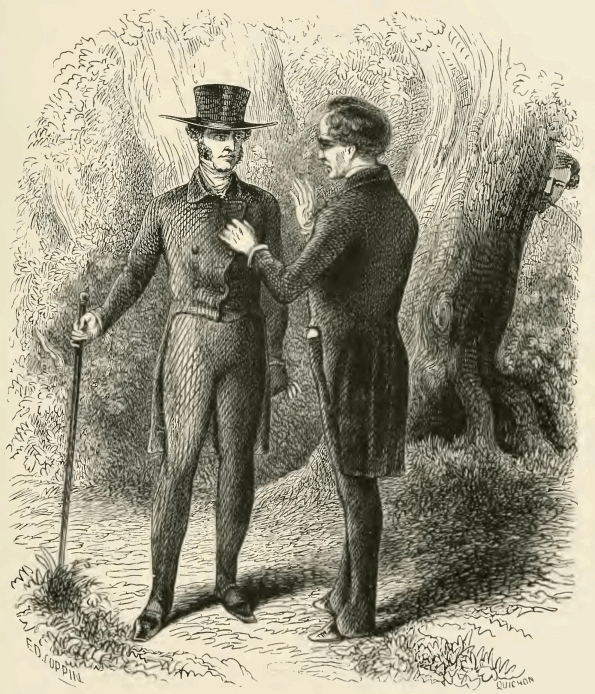
\includegraphics[width=\textwidth]{30345m.jpg}
\end{figure}

“But I do not think so.”

“Have pity on me doctor! So many dreadful things have happened to me
lately that I am on the verge of madness.”

“Has anyone besides me seen Madame de Saint-Méran?”

“No.”

“Has anything been sent for from a chemist’s that I have not examined?”

“Nothing.”

“Had Madame de Saint-Méran any enemies?”

“Not to my knowledge.”

“Would her death affect anyone’s interest?”

“It could not indeed, my daughter is her only heiress—Valentine alone.
Oh, if such a thought could present itself, I would stab myself to
punish my heart for having for one instant harbored it.”

“Indeed, my dear friend,” said M. d’Avrigny, “I would not accuse
anyone; I speak only of an accident, you understand,—of a mistake,—but
whether accident or mistake, the fact is there; it is on my conscience
and compels me to speak aloud to you. Make inquiry.”

“Of whom?—how?—of what?”

“May not Barrois, the old servant, have made a mistake, and have given
Madame de Saint-Méran a dose prepared for his master?”

“For my father?”

“Yes.”

“But how could a dose prepared for M. Noirtier poison Madame de
Saint-Méran?”

“Nothing is more simple. You know poisons become remedies in certain
diseases, of which paralysis is one. For instance, having tried every
other remedy to restore movement and speech to M. Noirtier, I resolved
to try one last means, and for three months I have been giving him
brucine; so that in the last dose I ordered for him there were six
grains. This quantity, which is perfectly safe to administer to the
paralyzed frame of M. Noirtier, which has become gradually accustomed
to it, would be sufficient to kill another person.”

“My dear doctor, there is no communication between M. Noirtier’s
apartment and that of Madame de Saint-Méran, and Barrois never entered
my mother-in-law’s room. In short, doctor although I know you to be the
most conscientious man in the world, and although I place the utmost
reliance in you, I want, notwithstanding my conviction, to believe this
axiom, \textit{errare humanum est}.”

“Is there one of my brethren in whom you have equal confidence with
myself?”

“Why do you ask me that?—what do you wish?”

“Send for him; I will tell him what I have seen, and we will consult
together, and examine the body.”

“And you will find traces of poison?”

“No, I did not say of poison, but we can prove what was the state of
the body; we shall discover the cause of her sudden death, and we shall
say, ‘Dear Villefort, if this thing has been caused by negligence,
watch over your servants; if from hatred, watch your enemies.’”

“What do you propose to me, d’Avrigny?” said Villefort in despair; “so
soon as another is admitted into our secret, an inquest will become
necessary; and an inquest in my house—impossible! Still,” continued the
procureur, looking at the doctor with uneasiness, “if you wish it—if
you demand it, why then it shall be done. But, doctor, you see me
already so grieved—how can I introduce into my house so much scandal,
after so much sorrow? My wife and my daughter would die of it! And I,
doctor—you know a man does not arrive at the post I occupy—one has not
been king’s attorney twenty-five years without having amassed a
tolerable number of enemies; mine are numerous. Let this affair be
talked of, it will be a triumph for them, which will make them rejoice,
and cover me with shame. Pardon me, doctor, these worldly ideas; were
you a priest I should not dare tell you that, but you are a man, and
you know mankind. Doctor, pray recall your words; you have said
nothing, have you?”

“My dear M. de Villefort,” replied the doctor, “my first duty is to
humanity. I would have saved Madame de Saint-Méran, if science could
have done it; but she is dead and my duty regards the living. Let us
bury this terrible secret in the deepest recesses of our hearts; I am
willing, if anyone should suspect this, that my silence on the subject
should be imputed to my ignorance. Meanwhile, sir, watch always—watch
carefully, for perhaps the evil may not stop here. And when you have
found the culprit, if you find him, I will say to you, ‘You are a
magistrate, do as you will!’”

“I thank you, doctor,” said Villefort with indescribable joy; “I never
had a better friend than you.” And, as if he feared Doctor d’Avrigny
would recall his promise, he hurried him towards the house.

When they were gone, Morrel ventured out from under the trees, and the
moon shone upon his face, which was so pale it might have been taken
for that of a ghost.

“I am manifestly protected in a most wonderful, but most terrible
manner,” said he; “but Valentine, poor girl, how will she bear so much
sorrow?”

As he thought thus, he looked alternately at the window with red
curtains and the three windows with white curtains. The light had
almost disappeared from the former; doubtless Madame de Villefort had
just put out her lamp, and the nightlamp alone reflected its dull light
on the window. At the extremity of the building, on the contrary, he
saw one of the three windows open. A wax-light placed on the
mantle-piece threw some of its pale rays without, and a shadow was seen
for one moment on the balcony. Morrel shuddered; he thought he heard a
sob.

It cannot be wondered at that his mind, generally so courageous, but
now disturbed by the two strongest human passions, love and fear, was
weakened even to the indulgence of superstitious thoughts. Although it
was impossible that Valentine should see him, hidden as he was, he
thought he heard the shadow at the window call him; his disturbed mind
told him so. This double error became an irresistible reality, and by
one of the incomprehensible transports of youth, he bounded from his
hiding-place, and with two strides, at the risk of being seen, at the
risk of alarming Valentine, at the risk of being discovered by some
exclamation which might escape the young girl, he crossed the
flower-garden, which by the light of the moon resembled a large white
lake, and having passed the rows of orange-trees which extended in
front of the house, he reached the step, ran quickly up and pushed the
door, which opened without offering any resistance.

Valentine had not seen him. Her eyes, raised towards heaven, were
watching a silvery cloud gliding over the azure, its form that of a
shadow mounting towards heaven. Her poetic and excited mind pictured it
as the soul of her grandmother.

Meanwhile, Morrel had traversed the anteroom and found the staircase,
which, being carpeted, prevented his approach being heard, and he had
regained that degree of confidence that the presence of M. de Villefort
even would not have alarmed him. He was quite prepared for any such
encounter. He would at once approach Valentine’s father and acknowledge
all, begging Villefort to pardon and sanction the love which united two
fond and loving hearts. Morrel was mad.

Happily he did not meet anyone. Now, especially, did he find the
description Valentine had given of the interior of the house useful to
him; he arrived safely at the top of the staircase, and while he was
feeling his way, a sob indicated the direction he was to take. He
turned back, a door partly open enabled him to see his road, and to
hear the voice of one in sorrow. He pushed the door open and entered.
At the other end of the room, under a white sheet which covered it, lay
the corpse, still more alarming to Morrel since the account he had so
unexpectedly overheard. By its side, on her knees, and with her head
buried in the cushion of an easy-chair, was Valentine, trembling and
sobbing, her hands extended above her head, clasped and stiff. She had
turned from the window, which remained open, and was praying in accents
that would have affected the most unfeeling; her words were rapid,
incoherent, unintelligible, for the burning weight of grief almost
stopped her utterance.

The moon shining through the open blinds made the lamp appear to burn
paler, and cast a sepulchral hue over the whole scene. Morrel could not
resist this; he was not exemplary for piety, he was not easily
impressed, but Valentine suffering, weeping, wringing her hands before
him, was more than he could bear in silence. He sighed, and whispered a
name, and the head bathed in tears and pressed on the velvet cushion of
the chair—a head like that of a Magdalen by Correggio—was raised and
turned towards him. Valentine perceived him without betraying the least
surprise. A heart overwhelmed with one great grief is insensible to
minor emotions. Morrel held out his hand to her. Valentine, as her only
apology for not having met him, pointed to the corpse under the sheet,
and began to sob again.

Neither dared for some time to speak in that room. They hesitated to
break the silence which death seemed to impose; at length Valentine
ventured.

“My friend,” said she, “how came you here? Alas, I would say you are
welcome, had not death opened the way for you into this house.”

“Valentine,” said Morrel with a trembling voice, “I had waited since
half-past eight, and did not see you come; I became uneasy, leaped the
wall, found my way through the garden, when voices conversing about the
fatal event——”

“What voices?” asked Valentine. Morrel shuddered as he thought of the
conversation of the doctor and M. de Villefort, and he thought he could
see through the sheet the extended hands, the stiff neck, and the
purple lips.

“Your servants,” said he, “who were repeating the whole of the
sorrowful story; from them I learned it all.”

“But it was risking the failure of our plan to come up here, love.”

“Forgive me,” replied Morrel; “I will go away.”

“No,” said Valentine, “you might meet someone; stay.”

“But if anyone should come here——”

The young girl shook her head. “No one will come,” said she; “do not
fear, there is our safeguard,” pointing to the bed.

“But what has become of M. d’Épinay?” replied Morrel.

\begin{figure}[ht]
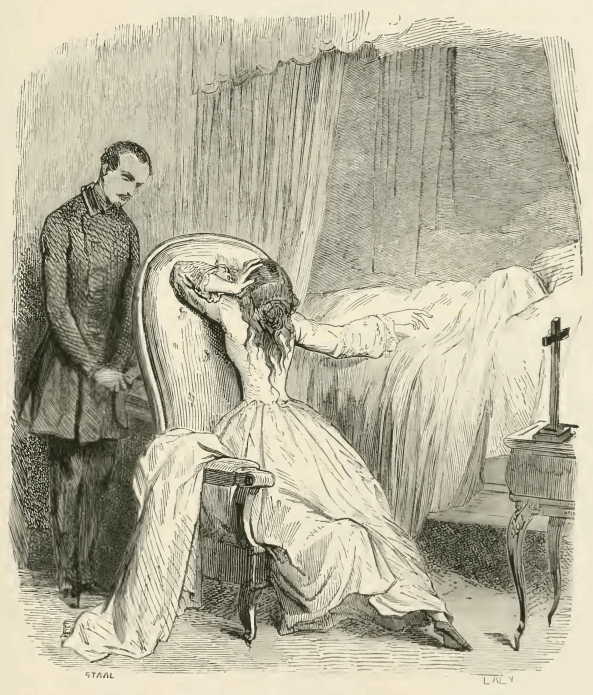
\includegraphics[width=\textwidth]{30349m.jpg}
\end{figure}

“M. Franz arrived to sign the contract just as my dear grandmother was
dying.”

“Alas,” said Morrel with a feeling of selfish joy; for he thought this
death would cause the wedding to be postponed indefinitely.

“But what redoubles my sorrow,” continued the young girl, as if this
feeling was to receive its immediate punishment, “is that the poor old
lady, on her death-bed, requested that the marriage might take place as
soon as possible; she also, thinking to protect me, was acting against
me.”

“Hark!” said Morrel. They both listened; steps were distinctly heard in
the corridor and on the stairs.

“It is my father, who has just left his study.”

“To accompany the doctor to the door,” added Morrel.

“How do you know it is the doctor?” asked Valentine, astonished.

“I imagined it must be,” said Morrel.

Valentine looked at the young man; they heard the street door close,
then M. de Villefort locked the garden door, and returned upstairs. He
stopped a moment in the anteroom, as if hesitating whether to turn to
his own apartment or into Madame de Saint-Méran’s; Morrel concealed
himself behind a door; Valentine remained motionless, grief seeming to
deprive her of all fear. M. de Villefort passed on to his own room.

“Now,” said Valentine, “you can neither go out by the front door nor by
the garden.”

Morrel looked at her with astonishment.

“There is but one way left you that is safe,” said she; “it is through
my grandfather’s room.” She rose. “Come,” she added.

“Where?” asked Maximilian.

“To my grandfather’s room.”

“I in M. Noirtier’s apartment?”

“Yes.”

“Can you mean it, Valentine?”

“I have long wished it; he is my only remaining friend and we both need
his help,—come.”

“Be careful, Valentine,” said Morrel, hesitating to comply with the
young girl’s wishes; “I now see my error—I acted like a madman in
coming in here. Are you sure you are more reasonable?”

“Yes,” said Valentine; “and I have but one scruple,—that of leaving my
dear grandmother’s remains, which I had undertaken to watch.”

“Valentine,” said Morrel, “death is in itself sacred.”

“Yes,” said Valentine; “besides, it will not be for long.”

She then crossed the corridor, and led the way down a narrow staircase
to M. Noirtier’s room; Morrel followed her on tiptoe; at the door they
found the old servant.

“Barrois,” said Valentine, “shut the door, and let no one come in.”

She passed first.

Noirtier, seated in his chair, and listening to every sound, was
watching the door; he saw Valentine, and his eye brightened. There was
something grave and solemn in the approach of the young girl which
struck the old man, and immediately his bright eye began to
interrogate.

\begin{figure}[ht]
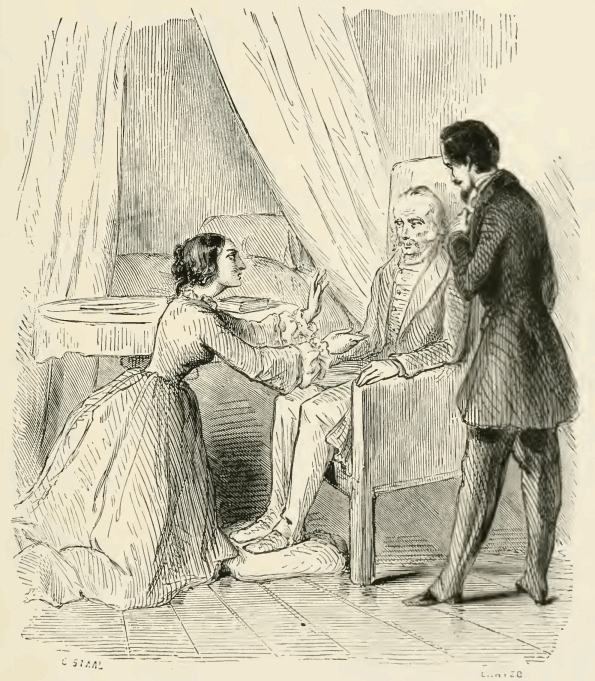
\includegraphics[width=\textwidth]{30351m.jpg}
\end{figure}

“Dear grandfather.” said she hurriedly, “you know poor grandmamma died
an hour since, and now I have no friend in the world but you.”

His expressive eyes evinced the greatest tenderness.

“To you alone, then, may I confide my sorrows and my hopes?”

The paralytic motioned “Yes.”

Valentine took Maximilian’s hand.

“Look attentively, then, at this gentleman.”

The old man fixed his scrutinizing gaze with slight astonishment on
Morrel.

“It is M. Maximilian Morrel,” said she; “the son of that good merchant
of Marseilles, whom you doubtless recollect.”

“Yes,” said the old man.

“He brings an irreproachable name, which Maximilian is likely to render
glorious, since at thirty years of age he is a captain, an officer of
the Legion of Honor.”

The old man signified that he recollected him.

“Well, grandpapa,” said Valentine, kneeling before him, and pointing to
Maximilian, “I love him, and will be only his; were I compelled to
marry another, I would destroy myself.”

The eyes of the paralytic expressed a multitude of tumultuous thoughts.

“You like M. Maximilian Morrel, do you not, grandpapa?” asked
Valentine.

“Yes.”

“And you will protect us, who are your children, against the will of my
father?”

Noirtier cast an intelligent glance at Morrel, as if to say, “perhaps I
may.”

Maximilian understood him.

“Mademoiselle,” said he, “you have a sacred duty to fulfil in your
deceased grandmother’s room, will you allow me the honor of a few
minutes’ conversation with M. Noirtier?”

“That is it,” said the old man’s eye. Then he looked anxiously at
Valentine.

“Do you fear he will not understand?”

“Yes.”

“Oh, we have so often spoken of you, that he knows exactly how I talk
to you.” Then turning to Maximilian, with an adorable smile; although
shaded by sorrow,—“He knows everything I know,” said she.

Valentine arose, placed a chair for Morrel, requested Barrois not to
admit anyone, and having tenderly embraced her grandfather, and
sorrowfully taken leave of Morrel, she went away. To prove to Noirtier
that he was in Valentine’s confidence and knew all their secrets,
Morrel took the dictionary, a pen, and some paper, and placed them all
on a table where there was a light.

“But first,” said Morrel, “allow me, sir, to tell you who I am, how
much I love Mademoiselle Valentine, and what are my designs respecting
her.”

Noirtier made a sign that he would listen.

It was an imposing sight to witness this old man, apparently a mere
useless burden, becoming the sole protector, support, and adviser of
the lovers who were both young, beautiful, and strong. His remarkably
noble and austere expression struck Morrel, who began his story with
trembling. He related the manner in which he had become acquainted with
Valentine, and how he had loved her, and that Valentine, in her
solitude and her misfortune, had accepted the offer of his devotion. He
told him his birth, his position, his fortune, and more than once, when
he consulted the look of the paralytic, that look answered, “That is
good, proceed.”

“And now,” said Morrel, when he had finished the first part of his
recital, “now I have told you of my love and my hopes, may I inform you
of my intentions?”

“Yes,” signified the old man.

“This was our resolution; a cabriolet was in waiting at the gate, in
which I intended to carry off Valentine to my sister’s house, to marry
her, and to wait respectfully M. de Villefort’s pardon.”

“No,” said Noirtier.

“We must not do so?”

“No.”

“You do not sanction our project?”

“No.”

“There is another way,” said Morrel. The old man’s interrogative eye
said, “Which?”

“I will go,” continued Maximilian, “I will seek M. Franz d’Épinay—I am
happy to be able to mention this in Mademoiselle de Villefort’s
absence—and will conduct myself toward him so as to compel him to
challenge me.” Noirtier’s look continued to interrogate.

“You wish to know what I will do?”

“Yes.”

“I will find him, as I told you. I will tell him the ties which bind me
to Mademoiselle Valentine; if he be a sensible man, he will prove it by
renouncing of his own accord the hand of his betrothed, and will secure
my friendship, and love until death; if he refuse, either through
interest or ridiculous pride, after I have proved to him that he would
be forcing my wife from me, that Valentine loves me, and will have no
other, I will fight with him, give him every advantage, and I shall
kill him, or he will kill me; if I am victorious, he will not marry
Valentine, and if I die, I am very sure Valentine will not marry him.”

Noirtier watched, with indescribable pleasure, this noble and sincere
countenance, on which every sentiment his tongue uttered was depicted,
adding by the expression of his fine features all that coloring adds to
a sound and faithful drawing.

Still, when Morrel had finished, he shut his eyes several times, which
was his manner of saying “No.”

“No?” said Morrel; “you disapprove of this second project, as you did
of the first?”

“I do,” signified the old man.

“But what then must be done?” asked Morrel. “Madame de Saint-Méran’s
last request was, that the marriage might not be delayed; must I let
things take their course?” Noirtier did not move. “I understand,” said
Morrel; “I am to wait.”

“Yes.”

“But delay may ruin our plan, sir,” replied the young man. “Alone,
Valentine has no power; she will be compelled to submit. I am here
almost miraculously, and can scarcely hope for so good an opportunity
to occur again. Believe me, there are only the two plans I have
proposed to you; forgive my vanity, and tell me which you prefer. Do
you authorize Mademoiselle Valentine to intrust herself to my honor?”

“No.”

“Do you prefer I should seek M. d’Épinay?”

“No.”

“Whence then will come the help we need—from chance?” resumed Morrel.

“No.”

“From you?”

“Yes.”

“You thoroughly understand me, sir? Pardon my eagerness, for my life
depends on your answer. Will our help come from you?”

“Yes.”

“You are sure of it?”

“Yes.” There was so much firmness in the look which gave this answer,
no one could, at any rate, doubt his will, if they did his power.

“Oh, thank you a thousand times! But how, unless a miracle should
restore your speech, your gesture, your movement, how can you, chained
to that armchair, dumb and motionless, oppose this marriage?” A smile
lit up the old man’s face, a strange smile of the eyes in a paralyzed
face.

“Then I must wait?” asked the young man.

“Yes.”

“But the contract?” The same smile returned. “Will you assure me it
shall not be signed?”

“Yes,” said Noirtier.

“The contract shall not be signed!” cried Morrel. “Oh, pardon me, sir;
I can scarcely realize so great a happiness. Will they not sign it?”

“No,” said the paralytic. Notwithstanding that assurance, Morrel still
hesitated. This promise of an impotent old man was so strange that,
instead of being the result of the power of his will, it might emanate
from enfeebled organs. Is it not natural that the madman, ignorant of
his folly, should attempt things beyond his power? The weak man talks
of burdens he can raise, the timid of giants he can confront, the poor
of treasures he spends, the most humble peasant, in the height of his
pride, calls himself Jupiter. Whether Noirtier understood the young
man’s indecision, or whether he had not full confidence in his
docility, he looked uneasily at him.

“What do you wish, sir?” asked Morrel; “that I should renew my promise
of remaining tranquil?” Noirtier’s eye remained fixed and firm, as if
to imply that a promise did not suffice; then it passed from his face
to his hands.

“Shall I swear to you, sir?” asked Maximilian.

“Yes,” said the paralytic with the same solemnity. Morrel understood
that the old man attached great importance to an oath. He extended his
hand.

“I swear to you, on my honor,” said he, “to await your decision
respecting the course I am to pursue with M. d’Épinay.”

“That is right,” said the old man.

“Now,” said Morrel, “do you wish me to retire?”

“Yes.”

“Without seeing Mademoiselle Valentine?”

“Yes.”

Morrel made a sign that he was ready to obey. “But,” said he, “first
allow me to embrace you as your daughter did just now.” Noirtier’s
expression could not be understood. The young man pressed his lips on
the same spot, on the old man’s forehead, where Valentine’s had been.
Then he bowed a second time and retired.

He found outside the door the old servant, to whom Valentine had given
directions. Morrel was conducted along a dark passage, which led to a
little door opening on the garden, soon found the spot where he had
entered, with the assistance of the shrubs gained the top of the wall,
and by his ladder was in an instant in the clover-field where his
cabriolet was still waiting for him. He got in it, and thoroughly
wearied by so many emotions, arrived about midnight in the Rue Meslay,
threw himself on his bed and slept soundly.
